\documentclass[11pt]{article}
\usepackage[margin=0.9in]{geometry}
\usepackage{amsmath,amssymb,booktabs,graphicx,float,array,xcolor}
\usepackage[hidelinks]{hyperref}
\usepackage{caption}
\captionsetup{font=small}
\setlength{\parskip}{3pt}
\setlength{\parindent}{0pt}
\newcommand{\thw}{\tilde\theta}

\title{COSC 527 Midterm Project A:\\ Swing-Up and Balancing of a Furuta Pendulum with Tabular RL}
\author{Joshua Stenger}
\date{\today}

\begin{document}
\maketitle

\noindent Every number in this report is printed by the submitted scripts and saved in
\texttt{results/}. All figures are generated by \texttt{stenger\_midterm\_experiment.py}.
The supplied simulator \texttt{futura\_env/furuta\_env.py} is used \emph{unmodified and
unwrapped}: the agent only calls its constructor, \texttt{reset()} and \texttt{step()}.

\section{Problem, environment, and the two stages}

The state is $x=[\phi,\dot\phi,\theta,\dot\theta]^T$ (arm angle and rate, pendulum angle and
rate). The agent selects one of three actions, which apply the torques
$\{-0.02,0,+0.02\}$\,N\,m; the environment integrates the G\"afvert (1998) model with RK4 at
$T_s=0.01$\,s. Table~\ref{tab:env} lists the values defined in the supplied file
(\texttt{results/part1\_environment.txt}).

\begin{table}[H]\centering\small
\begin{tabular}{ll}\toprule
Quantity & Value in \texttt{furuta\_env.py}\\\midrule
Sampling time, horizon & $T_s=0.01$\,s, \texttt{max\_steps}$=2000$ (20\,s) $\Rightarrow$ \texttt{truncated}\\
Pendulum limit & \texttt{angle\_limit}$=20^\circ$ on the \emph{raw} $\theta$ $\Rightarrow$ \texttt{terminated}\\
Arm safety limit & \texttt{arm\_angle\_limit}$=\pi$: $|\phi|>\pi\Rightarrow$ \texttt{terminated} (no velocity limit exists in the file)\\
Built-in reward & $1-(\theta/0.349)^2-0.001u^2$, and $-10$ on termination\\
Default \texttt{reset()} & $\phi_0,\theta_0\sim U(-0.02,0.02)$\,rad, rates $0$ (near \emph{upright})\\\bottomrule
\end{tabular}
\caption{Environment facts, read from the supplied file.}\label{tab:env}
\end{table}

\textbf{Interface checks.} The supplied \texttt{example\_run.py} (zero torque, seed 7) falls
after 55 steps with return 36.89. From the same state, actions 0/1/2 report torques
$-0.020/0.000/+0.020$, and action 3 raises \texttt{ValueError}. In the swing-up configuration,
one continuing transition from $\thw_0=-178.75^\circ$ with $A=2$ gives $R=-1.00015$, not
terminal. All three outcomes appear: a constant $+0.02$ torque from the bottom violates the
arm limit after 107 steps (\emph{unsafe}); \texttt{max\_steps=50} returns
\texttt{(terminated, truncated)=(False, True)} (\emph{time limit}); and a 500-step upright hold
(\emph{success}) is detected by the agent's counter. The \textbf{agent} chooses $A_t$ and owns the
discretization, the Q table, $\epsilon,\alpha,\gamma$, the swing-up reward and the success counter. The
\textbf{environment} produces $S_{t+1}$, the applied torque, its built-in reward, and the
\texttt{terminated}/\texttt{truncated} flags.

\textbf{Two stages (as instructed).} \emph{Stage~1 (balance, no swing-up)} uses
\texttt{FurutaEnv()} with every default, including its reward and its $20^\circ$ termination. This
answers whether the agent can stabilize the pendulum at all. \emph{Stage~2 (swing-up)} is the
project task, set up through public arguments only:
\begin{itemize}
\item \texttt{FurutaEnv(angle\_limit=np.inf)}, because the PDF requires that leaving the upright
region must not end the episode (the default would terminate on the very first step from
the bottom);
\item \texttt{reset(initial\_state=[0,\dot\phi_0,\pi+\alpha,\dot\theta_0])} with
$\alpha\sim U(-5^\circ,5^\circ)$ and $\dot\phi_0,\dot\theta_0\sim U(-0.05,0.05)$;
\item the arm limit $\pi$ and \texttt{max\_steps}$=2000$ are kept unchanged.
\end{itemize}
Because the supplied reward is only defined for balancing (it becomes constant when
\texttt{angle\_limit}$=\infty$), the agent computes the project's baseline reward from the observed
$S_{t+1}$ and \texttt{info["torque"]}:
\[
R_{t+1}=\cos\thw_{t+1}-\lambda_\phi\phi_{t+1}^2-\lambda_u u_t^2\;(+100\text{ on success}),\qquad
\lambda_\phi=0.1,\ \lambda_u=1,\qquad R=-200\text{ on an unsafe termination}.
\]
The $-200$ penalty is needed because rewards near the bottom are about $-1$ per step. Without it,
ending the episode early by hitting the arm limit would be \emph{better} than continuing to swing
($\sum\gamma^k(-1)\approx-100$). Success means $|\thw|\le 20^\circ$ for 500 consecutive simulator
steps. The counter resets whenever the pendulum leaves the region, and success ends the episode
as a terminal transition.

\section{Finite state representation}

Bins are internal edges passed to the supplied \texttt{discretize\_state} convention (a value on
an edge goes to the upper bin; values outside the outermost edges fall into the end bins). The
angle is wrapped first, $\thw=\mathrm{wrapToPi}(\theta)$. For speed the agent uses an equivalent
\texttt{bisect} lookup, and the verification script checks it against the supplied helper on
5000 random states per table.

\begin{table}[H]\centering\small
\begin{tabular}{lll}\toprule
 & Stage 1: balance (5$\times$6$\times$10$\times$10) & Stage 2: swing-up (7$\times$8$\times$18$\times$14)\\\midrule
$\phi$ (rad) & $\pm0.3,\pm1$ & $\pm0.3,\pm1,\pm2$\\
$\dot\phi$ (rad/s) & $0,\pm0.3,\pm1.5$ & $0,\pm0.3,\pm1.5,\pm3$\\
$\thw$ (deg) & $0,\pm1,\pm3,\pm6,\pm12$ & $0,\pm1,\pm3,\pm6,\pm12,\pm20,\pm45,\pm90,\pm135$\\
$\dot\theta$ (rad/s) & $0,\pm0.1,\pm0.4,\pm1,\pm2$ & $0,\pm0.1,\pm0.4,\pm1,\pm2,\pm4,\pm8$\\\midrule
$|\mathcal S|$, $|\mathcal S||\mathcal A|$ & 3000 states, \textbf{9000} entries & 14\,112 states, \textbf{42\,336} entries\\\bottomrule
\end{tabular}
\caption{Interior bin edges and table sizes (\texttt{results/part2\_discretization.txt}).}\label{tab:bins}
\end{table}

\textbf{Rationale.} A torque of $0.02$\,N\,m can only hold the pendulum against gravity up to
roughly $8.7^\circ$ (linearized $\ddot\theta=47.9\theta-365u$), so the balancing bins are
concentrated inside $\pm12^\circ$ with fine rate bins. The swing-up table keeps exactly these
near-upright edges, so the catch can be represented. It adds coarse $\thw$ bins covering the full
$[-\pi,\pi]$ range (the downward position falls in the end bins, $|\thw|>135^\circ$), and $\dot\theta$
bins up to $\pm8$\,rad/s for the large motions of the swing. The arm bins reach $\pm2$\,rad,
because a feasible swing-up needs about $\pm1.8$\,rad of arm travel. Values below, inside, and
above every range were tested (e.g.\ $\dot\phi=10^6\mapsto$ the last bin, $\theta=3\pi/2\mapsto
\thw=-\pi/2$), and every index is valid.

\section{Action-value control, training, and evaluation}

\textbf{Updates.} The two methods use separate episode loops and separate target functions
(\texttt{stenger\_midterm\_agent.py}):
\[
\text{SARSA: } Y=R+\gamma Q(S',A'),\ A'\sim\epsilon\text{-greedy}(S')\text{ drawn \emph{before} the update and then executed};\qquad
\text{Q-learning: } Y=R+\gamma\max_a Q(S',a),
\]
with $Q(S,A)\leftarrow Q(S,A)+\alpha(Y-Q(S,A))$, and continuation value $0$ on terminal transitions
(unsafe or success). A time-limit truncation is not terminal: the target still bootstraps,
because the pendulum's state does not end at 20\,s. The behavior policy is $\epsilon$-greedy over
all three actions. Ties among maximizing actions are broken uniformly at random using the
seeded generator.

\textbf{Control interval.} The agent's decisions are the transitions the update rule sees.
Stage~1 decides every 10\,ms. In Stage~2 a single 10\,ms interval failed: after 1500 episodes the
pendulum never entered the upright region, because with the action changing every 10\,ms
the action values differ by almost nothing compared with their noise. Holding the action for
5 steps (50\,ms) produced clear energy pumping, but that rate cannot balance: a diagnostic Stage-1
run with 50\,ms decisions never exceeded a 1.7\,s hold. The final swing-up agent therefore acts
every 10\,ms when $|\thw|<25^\circ$ and every 50\,ms otherwise. The reward over a held action is the
sum of the per-step rewards, and the success and safety checks still run on every 10\,ms step.

\begin{table}[H]\centering\small
\begin{tabular}{lcc}\toprule
 & Stage 1 (balance) & Stage 2 (swing-up)\\\midrule
$\alpha$, $\gamma$ (per decision) & 0.1, 0.99 & 0.1, 0.99\\
$\epsilon$ schedule & $1\to0.01$ linearly over first 70\% of episodes & same\\
$Q_0$ (explicit initialization) & 100 (optimistic) & 0\\
Episodes per run (stopping criterion) & 2000 & 6000\\
Training seeds / evaluation seeds & 0,1,2 / 10000--10019 & same\\\bottomrule
\end{tabular}
\caption{Hyperparameters (all are dataclass fields in \texttt{Task}/\texttt{Hyper}).}\label{tab:hyper}
\end{table}

$Q_0$ differs because the reward scales differ. In Stage~1, rewards are about $+1$ per step, so
$Q_0=100\approx1/(1-\gamma)$ is optimistic and pushes systematic exploration (with $Q_0=0$ only 6 and 13
of 20 evaluation episodes succeeded in a pilot run). In Stage~2, $Q_0=0$ is already optimistic near
the bottom, where true values are about $-100$. A pilot with $Q_0=100$ never learned to hold the
pendulum, because it made falling look as valuable as staying up.

\textbf{Evaluation} uses a frozen copy of $Q$ (\texttt{setflags(write=False)}) with a greedy policy
($\epsilon=0$) and no updates. It runs 20 episodes from the controlled initial conditions given by
evaluation seeds 10000--10019, the same seeds for both methods and all experiments. Episodes that
never reach upright are reported as such, not discarded. The learned tables are saved in
\texttt{results/<experiment>\_<method>\_seed<k>.npz}.

\section{Results}

\subsection*{Stage 1: balancing with the supplied environment}

\begin{figure}[H]\centering
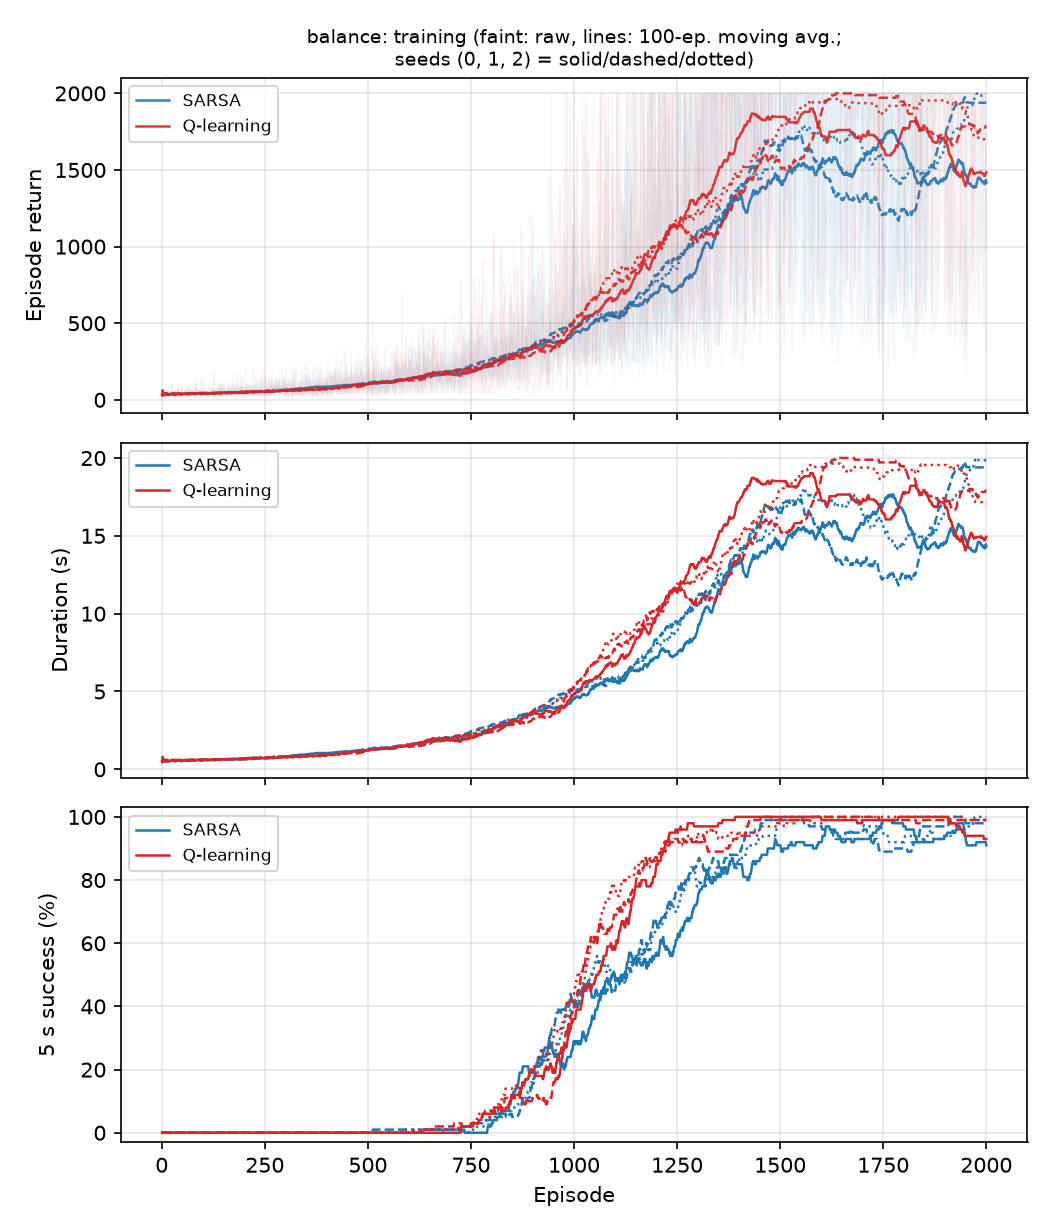
\includegraphics[width=0.62\linewidth]{figures/balance_training.png}
\caption{Stage 1 training: return, duration, and 5\,s success rate (100-episode moving average,
three seeds per method).}\label{fig:baltrain}
\end{figure}

\begin{table}[H]\centering\small
\begin{tabular}{lcccc}\toprule
Greedy evaluation, $3\times20$ episodes & 5\,s success & return (mean $\pm$ sd) & duration & full 20\,s\\\midrule
SARSA & \textbf{60/60} & $1901.9\pm296.4$ & 19.04\,s & 54/60\\
Q-learning & \textbf{60/60} & $1981.5\pm141.9$ & 19.82\,s & 59/60\\\bottomrule
\end{tabular}
\caption{Stage 1 evaluation. The episode starts upright, so the time to first enter the upright
region is one step (0.01\,s).}\label{tab:bal}
\end{table}

\textbf{The pendulum can be stabilized.} Both methods learn a balancing policy that holds for
5\,s from every evaluation start, and usually for the full 20\,s (Fig.~\ref{fig:baltrain}, Table~\ref{tab:bal}).
Training success rises from 0 near episode 750 to above 90\% by episode 1500. In the last 10\% of
training, Q-learning succeeds 96.5--99.5\% of the time and SARSA 92.5--97.5\%. SARSA learns a
slightly more cautious policy because its target includes its own exploratory actions. Its only
failures are 6 falls (after 8.4\,s or more) for seed~0.

\subsection*{Stage 2: swing-up and balancing (baseline reward)}

\begin{figure}[H]\centering
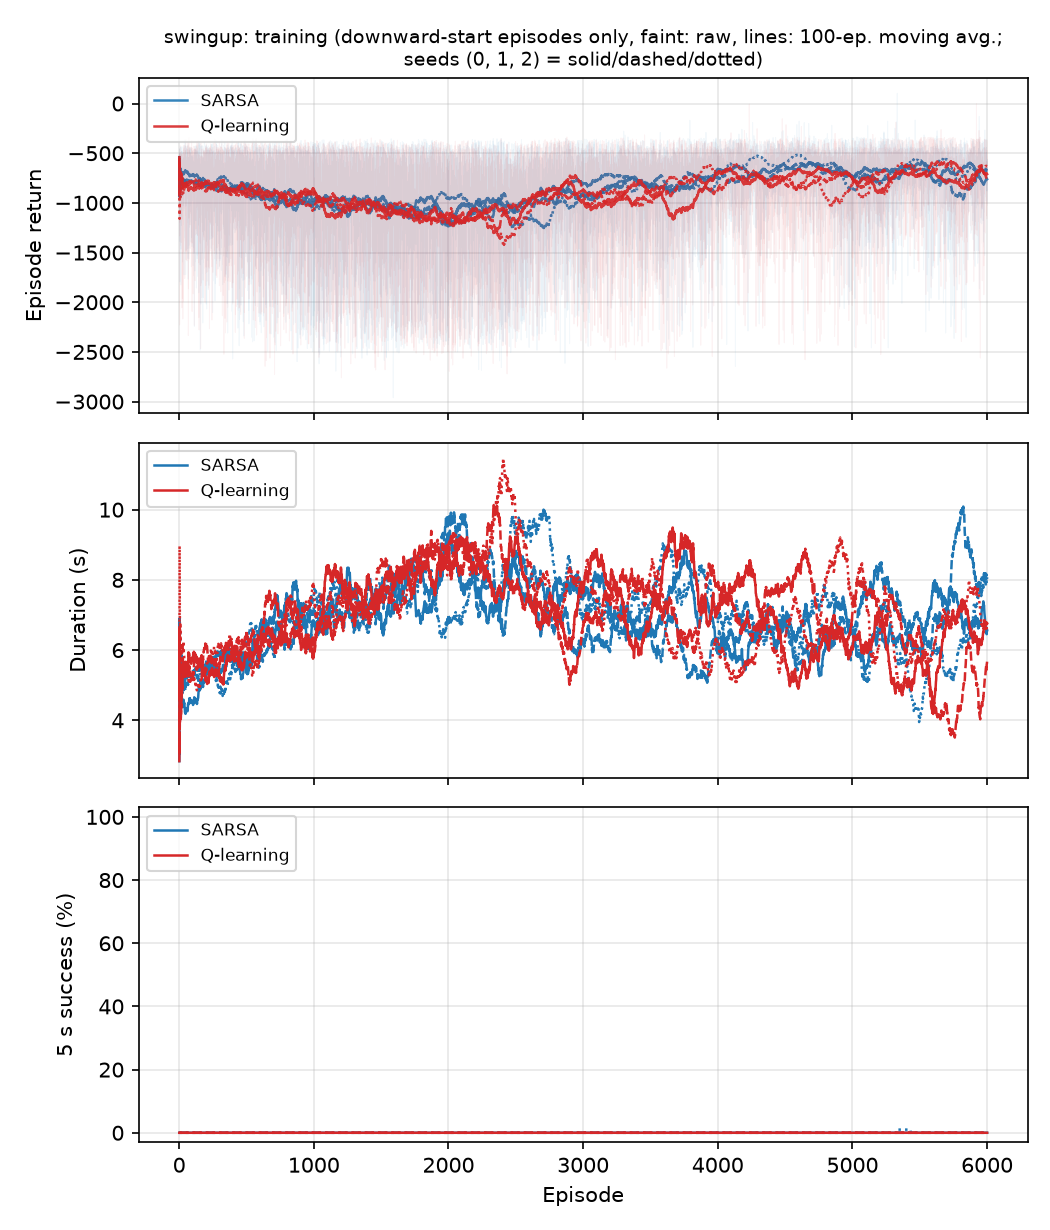
\includegraphics[width=0.49\linewidth]{figures/swingup_training.png}\hfill
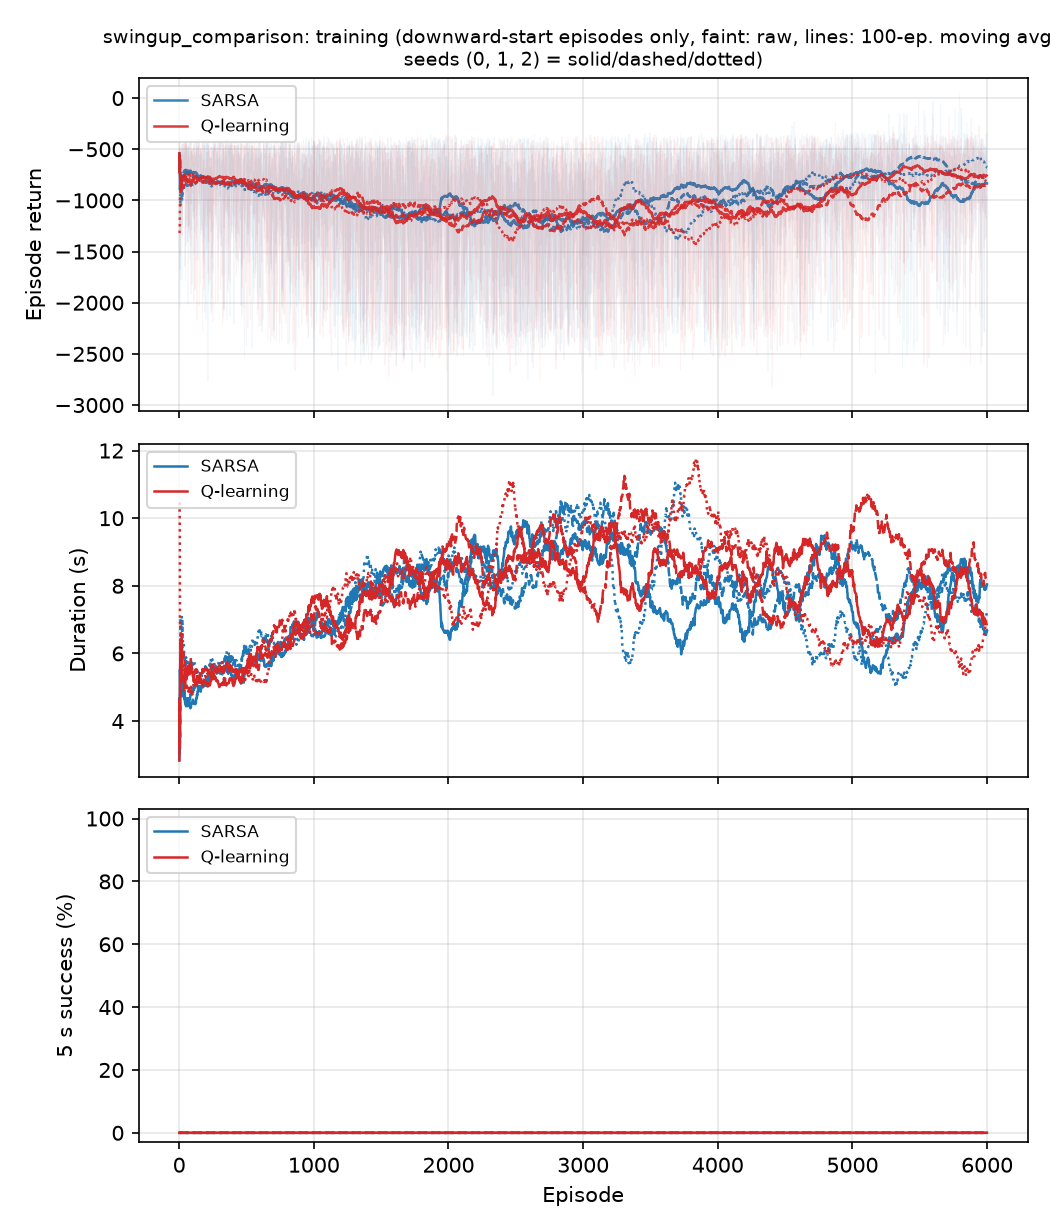
\includegraphics[width=0.49\linewidth]{figures/swingup_comparison_training.png}
\caption{Stage 2 training, downward-start episodes only. Left: baseline. Right: controlled
comparison with exploring starts (described below).}\label{fig:swtrain}
\end{figure}

\begin{figure}[H]\centering
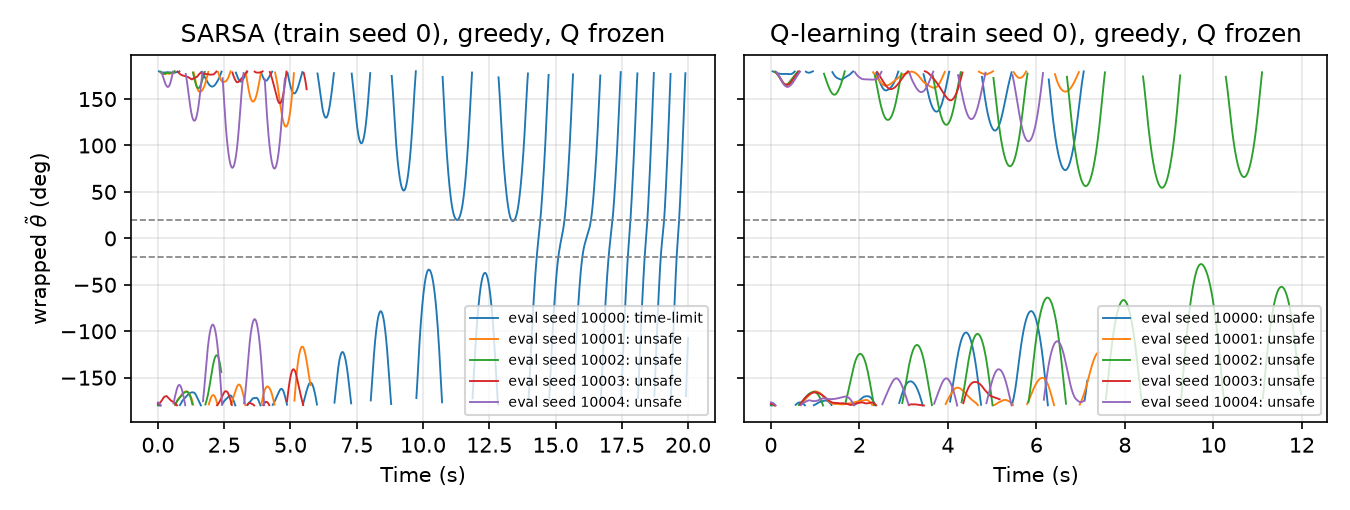
\includegraphics[width=0.85\linewidth]{figures/swingup_eval_theta.png}
\caption{Wrapped pendulum angle in five greedy evaluation episodes (baseline, training seed 0).
Dashed lines mark the $\pm20^\circ$ upright region.}\label{fig:theta}
\end{figure}

\begin{table}[H]\centering\small
\begin{tabular}{lccccccc}\toprule
Greedy eval., $3\times20$ ep. & success & return & reached upright & time to upright & duration & longest hold & outcome\\\midrule
SARSA & 0/60 & $-750.6\pm322.6$ & 15/60 & 7.57\,s & 7.97\,s & 0.55\,s & 57 unsafe, 3 time limit\\
Q-learning & 0/60 & $-731.2\pm170.9$ & 4/60 & 7.92\,s & 6.22\,s & 0.40\,s & 60 unsafe\\\bottomrule
\end{tabular}
\caption{Stage 2 baseline evaluation. Time to upright is averaged over the episodes that reached
it; the remaining 45/60 (SARSA) and 56/60 (Q-learning) \emph{never} came within $20^\circ$.}\label{tab:sw}
\end{table}

\textbf{Swing-up is learned only partially.} The agent learns to inject energy. The greedy swings
grow from $\pm5^\circ$ to over-the-top rotations within 5--10\,s (Fig.~\ref{fig:theta}), and
SARSA's policies reach the upright region in 15 of 60 evaluation episodes. However, \textbf{no
policy catches the pendulum}. Every arrival is too fast, the pendulum passes through the upright
region (the longest hold is 0.55\,s), and in 117 of 120 episodes the swinging eventually drives the
arm past $\pm\pi$. No 5\,s success is claimed. Training curves
(Fig.~\ref{fig:swtrain}) improve only slowly after episode 3000. SARSA reaches upright more often
than Q-learning (15 vs.\ 4). A plausible explanation is that its
on-policy targets include the exploratory torque reversals, which makes it more willing to keep
pumping and less willing to commit to a single direction that ends at the arm limit.

\subsection*{Controlled comparison: exploring starts}\label{sec:comp}

\textbf{Change made (only this one):} half of the \emph{training} episodes start from the supplied
\texttt{env.reset()} (near upright) instead of from the bottom. The reward, bins, control interval,
hyperparameters, seeds, and evaluation (always from the bottom) are identical. \textbf{Why:} the
baseline policies reach the top but cannot hold it, and the visit counts show why. Only 3.5--5.9\%
of decisions occur within $20^\circ$ of upright, so the balancing part of the table is barely trained.
Exploring starts (Sutton \& Barto, \S5.3) target exactly that gap, and they implement the
``stabilize first, then swing up'' idea inside one table.

\begin{figure}[H]\centering
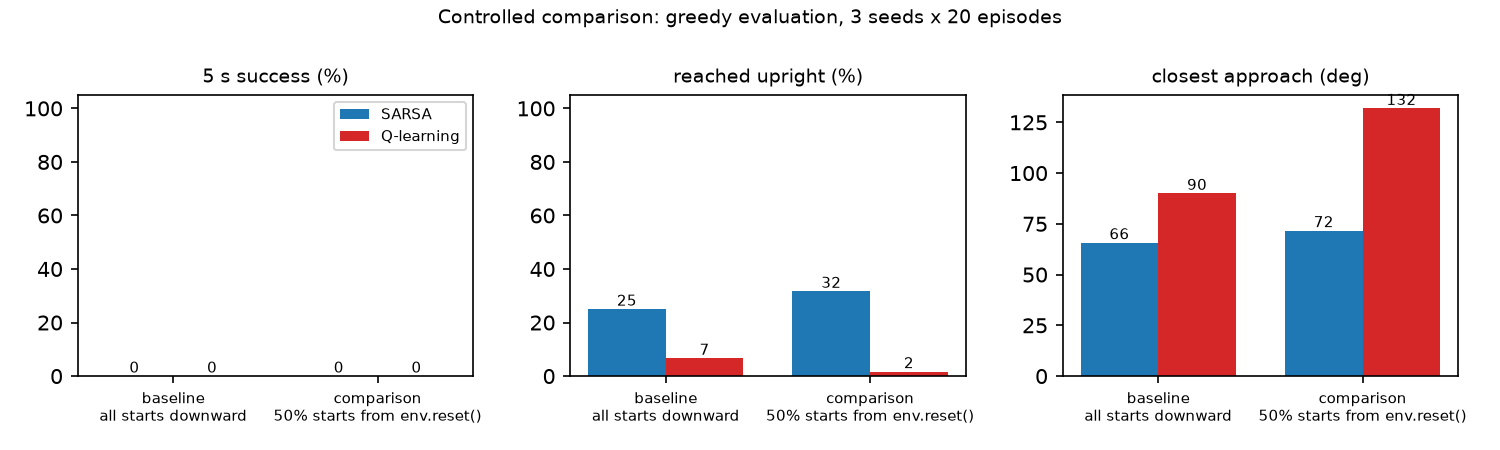
\includegraphics[width=0.9\linewidth]{figures/comparison.png}
\caption{Baseline vs.\ exploring starts, greedy evaluation from the bottom.}\label{fig:comp}
\end{figure}

\textbf{Effect.} Training return improves strongly: the last-10\% mean rises from about $-700$ to
$-210$ to $-430$. Within the upright-start training episodes, 14--48\% now succeed, so the table
\emph{did} learn to balance once it is at the top. The share of decisions within $20^\circ$ of upright
rises to 44--51\%. Evaluation from the bottom, however, does not improve. SARSA reaches upright
in 19/60 episodes (vs.\ 15/60), with the longest hold 1.12\,s. Q-learning drops to 1/60, and its
average closest approach worsens from $90^\circ$ to $132^\circ$. No downward-start episode succeeded in
training or in evaluation. \textbf{Interpretation:} the balancing skill is learned for states
near rest at the top, but a swing-up arrives with $|\dot\theta|$ of several rad/s, a region the upright
starts never visit. Half as many downward episodes also means half as much swing-up training,
which hurts Q-learning's greedy swing most. The comparison shows that the failure lies in
connecting the two phases (arriving slowly enough to be caught), not in the balancing skill
itself.

\section{Interpretation of the learned behavior}

\textbf{(a) Model-free.} The simulator integrates a model, but the agent never calls
\texttt{dynamics()} or \texttt{\_rk4()}. It never predicts alternative outcomes and never plans.
It only receives sampled tuples $(S_t,A_t,R_{t+1},S_{t+1})$ through \texttt{step()} and updates
$Q$ from them. The model lives inside the environment, not inside the agent.

\textbf{(b) Target policies.} SARSA's target policy is its behavior policy (the $\epsilon$-greedy
policy, on-policy), so it uses $Q(S',A')$ for the action actually taken next. Q-learning's target
policy is the greedy policy (off-policy), so it uses $\max_aQ(S',a)$ whatever is executed. For
the same sampled swing-up transition (\texttt{results/summary.txt}),
$Q(S',\cdot)=[-109.441,-109.578,-108.786]$, $R=-0.9989$, and $A'=1$ (exploratory). This gives
$Y_{\text{SARSA}}=-109.481$ and $Y_{\text{Q}}=-108.697$. The targets coincide only when $A'$ is greedy, and
both equal $R$ on terminal transitions.

\textbf{(c) Visitation.} In the swing-up baseline, 75--80\% of decisions occur with
$|\thw|>135^\circ$, i.e.\ hanging down, versus 3.5--5.9\% within $20^\circ$ of upright
(Fig.~\ref{fig:visits}). The visits are spread over all $\dot\theta$ bins up to $\pm8$\,rad/s, while 5069
(SARSA) and 5472 (Q-learning) of the 14\,112 states were never visited. In Stage~1, 79--88\% of
visits fall in the two $|\dot\theta|<0.1$ bins, and 1848--2022 of 3000 states are never visited.
This shows the discretization spends most of its resolution where the agent rarely goes:
the fine upright bins are almost unused during swing-up, while the bottom of the swing is
represented by only two coarse $\thw$ bins that hold most of the data.

\begin{figure}[H]\centering
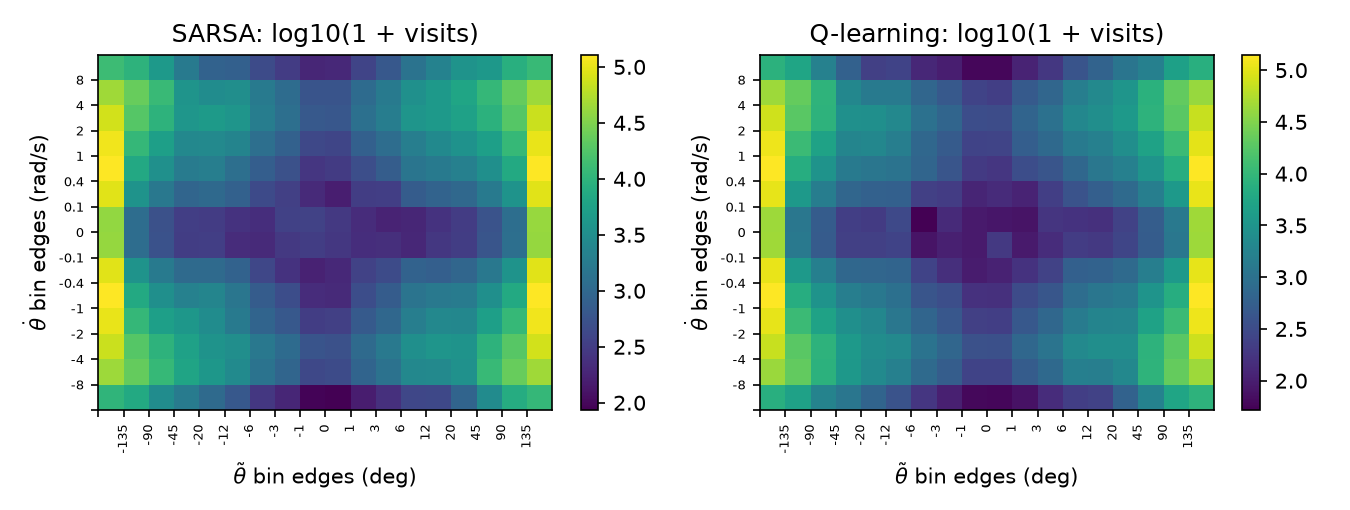
\includegraphics[width=0.75\linewidth]{figures/swingup_visits.png}
\caption{Visits per $(\thw,\dot\theta)$ cell, summed over $\phi,\dot\phi$ and three seeds (baseline swing-up).}\label{fig:visits}
\end{figure}

\textbf{(d) Larger training return $\ne$ better greedy policy.} Exploring starts improved
Q-learning's training return from about $-700$ to $-210$ to $-400$, yet its greedy evaluation from
the bottom got worse (upright 4/60 $\to$ 1/60, closest approach $90^\circ\to132^\circ$). The higher
training return came from easy upright-start episodes and from exploration, not from a better
swing-up policy. Within Stage~1, SARSA seed~0 had the lowest training return and also the only
evaluation falls. That agreement is not guaranteed in general.

\textbf{(e) Reward design.} $\cos\thw$ rises monotonically from $-1$ to $+1$ as the pendulum
climbs, so every swing that ends higher earns more reward. That rewards energy accumulation
long before the top is reached. Near upright, $\cos\thw\approx1$ is the largest per-step reward, and
the 500-step success bonus favors staying there. The arm penalty $\lambda_\phi\phi^2$ and the unsafe
penalty discourage solutions that wind the arm up. The weakness we observed: $\cos$ is almost
flat near the top ($\cos 10^\circ=0.985$), so it barely distinguishes a controllable arrival from a
fast pass-through.

\textbf{(f) Transfer to a QUBE-Servo 3.} The parameters are G\"afvert's, not the QUBE's, and the
model has no friction, motor dynamics, sensor noise, encoder quantization, or delay. A tabular
bang-bang policy that switches between $\pm0.02$\,N\,m every 10\,ms would chatter on real hardware,
and it would need to be retrained or fine-tuned on the actual plant.

\section{Limitations and lessons learned}

\begin{itemize}
\item The supplied environment has no swing-up reward and no success flag. The swing-up reward,
success counter, and initial condition are therefore implemented in the agent through the
public API. The environment itself was not modified, wrapped, or subclassed.
\item The choice of control interval decided whether learning worked at all: 10\,ms for balancing, 50\,ms
for pumping. The adaptive interval is a design decision of this project, not of the PDF.
\item With 14\,112 states and one-step targets, value information propagates slowly across the
$\sim$500-step swing, so 6000 episodes were not enough to learn the catch. Eligibility traces,
function approximation, or a finer table in the arrival region (high $|\dot\theta|$ near upright)
are the natural next steps.
\item Lesson: the start distribution decides what the table learns. Stage~1 succeeded because
the supplied start already lies in the tiny region where $\pm0.02$\,N\,m can recover. A wider
pilot start distribution ($\pm10^\circ$) made the same learner fail completely.
\end{itemize}

\appendix
\section{Use of generative AI}

\textbf{Tool:} Claude Code (Anthropic, model Claude Opus 5.5).

\textbf{Prompts:} ``copy assignment2 and build off of it for the midterm \ldots\ look at the pdfs in
the midterm folder and complete the project. Try to learn without the swing up first and see if
you can stabilize the pendulum. Then try with the swing-up.'' From HW2, this carried a standing
instruction: ``we should not be wrapping or editing the environment in any way shape or form.''

\textbf{How it influenced the work:} the tool drafted the agent, the scripts, the experiment design,
this report, and the slides, and it ran the pilot experiments summarized in Section~3.

\textbf{Suggestions verified, corrected, or rejected:}
\begin{itemize}
\item Rejected: wrapping \texttt{FurutaEnv} in a class that changes the reward and termination.
Only constructor arguments, \texttt{reset(initial\_state=...)} and \texttt{step()} are used.
\item Corrected: the first swing-up design (decisions every 10\,ms, $\epsilon$ from 1) never
approached upright. The tool's first fix (50\,ms decisions everywhere) swung up but could not
balance, which led to the adaptive interval.
\item Corrected: the first exploring-start distribution ($\thw\sim U(-10^\circ,10^\circ)$, rates up
to 0.5\,rad/s) was mostly unrecoverable; it was replaced by the supplied \texttt{reset()}.
\item Verified: the fast \texttt{bisect} discretizer against the supplied \texttt{discretize\_state}
on 5000 random states; the SARSA and Q-learning targets against hand-computed values; and
reproducibility (re-evaluating the saved tables gives identical numbers).
\end{itemize}

\textbf{Portions assisted:} all source files except the supplied \texttt{futura\_env/}; this report;
\texttt{slides/slides.tex}. I am responsible for checking and being able to explain every part.

\end{document}
